\section{应用场景展望}
在设计通证模型的时,为了尊重资产的公平性,正当性,确权性,使得在通证增发和分发模型的设计当中更为简单、透明、有效。结合星云的生态特点,我们将更多的激励和博弈场景交给了应用场景本身。例如:应用场景中的激励和消耗场景可以是变化、多样、有趣的。在这个章节当中,我们会针对星云中已经存在的或是将要发生的场景进行一些展望,通过对主要应用场景的展望,如图\ref{fig:nax_ecosys}所示,可以比较清晰的勾勒出NAX在星云生态的串联作用。

\begin{figure}[htbp]
  \centering
    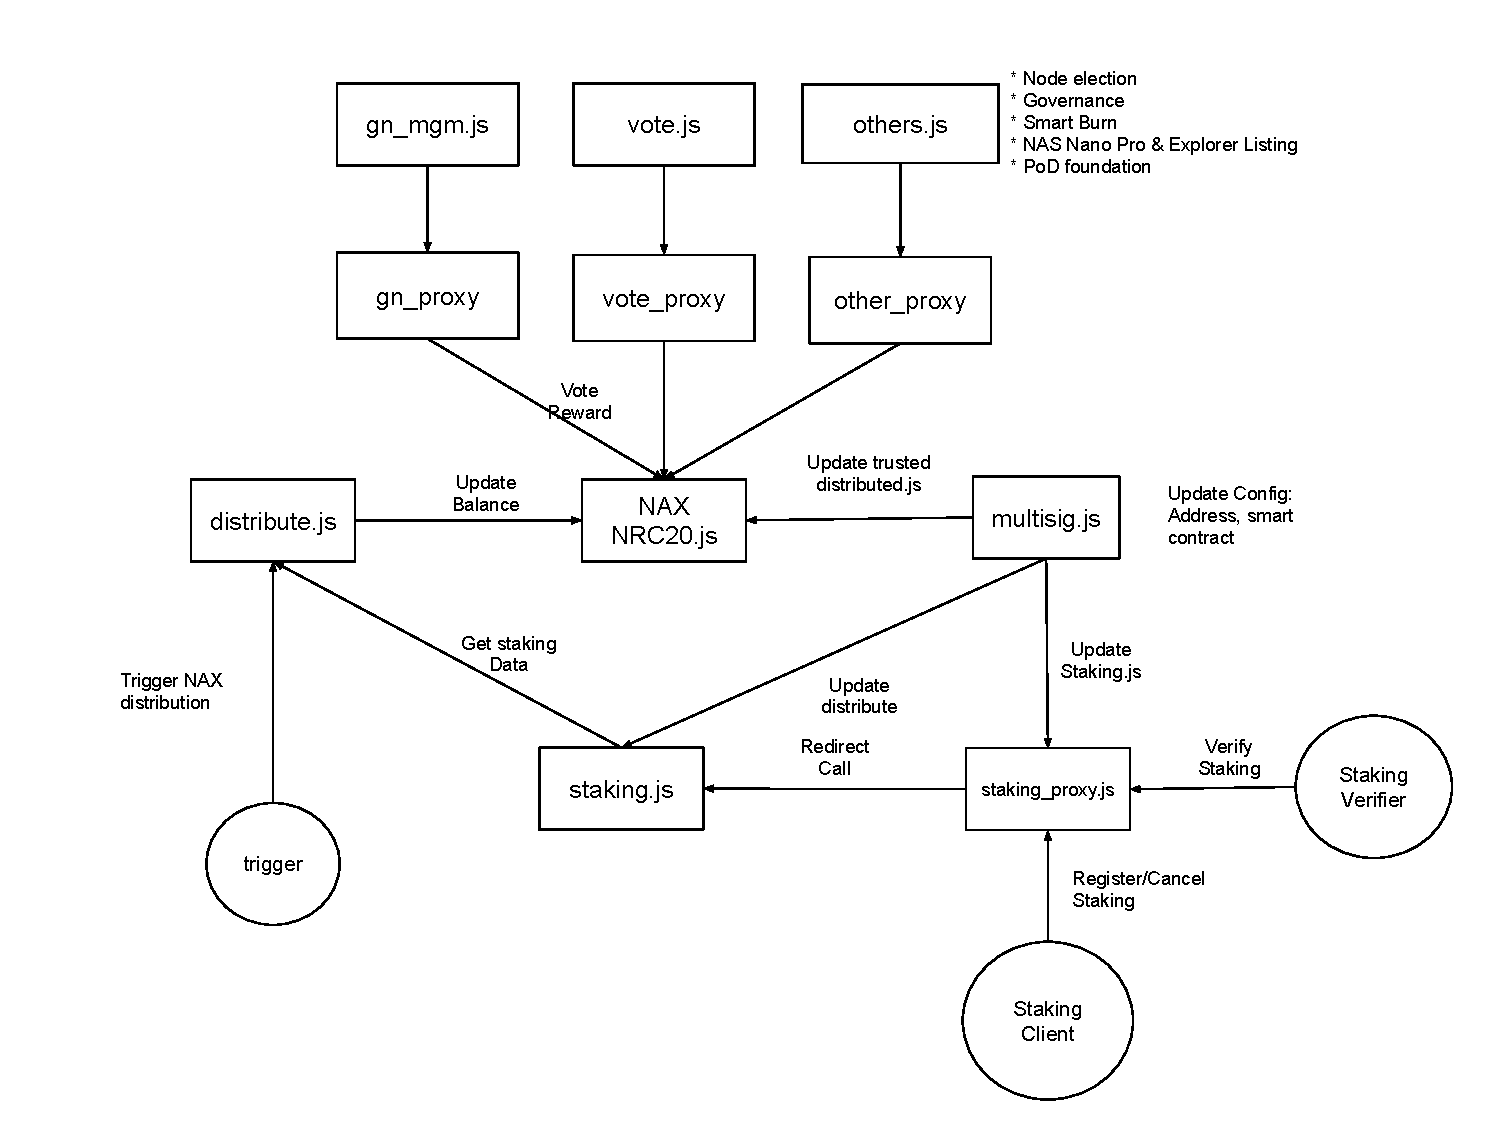
\includegraphics[width=1\textwidth]{../common/nax.pdf}
    \caption{NAX use-cases in Nebulas Ecosys \label{fig:nax_ecosys}}
\end{figure}

\subsection{生态贡献激励}
在白皮书中,从贡献证明的共识算法(PoD, Proof of Devotion),到星云的愿景的提出:在去中心化的协作中公平受益,再到2019年初,Go Nebulas平台的上线,都始终贯穿着星云对生态贡献度衡量的探索。这些都是星云进一步朝着Autonomous Metanet目标前进的重要环节。我们为此,提出一种以质押投资基金为权益证明的激励方式,使之运用到不同场景的激励当中。具体的操作是,将项目投资基金(通常以NAS形式存在),将这份基金进行质押,这部分资金质押所得的NAX权益,将作为该生态场景的NAX激励权益基金。

\subsubsection{Go Nebulas激励}
星云基金会将会投入不少于300万NAS的资金,用于资助Go Nebulas平台上的项目,而且根据需求,基金会也将随时追加资金的投入。这部分资金可以投入到质押当中,产生的权益将用来激励在Go Nebulas平台上做出大大小小贡献的证明,即在获得NAS资金作为报酬之外,还将获得由Go Nebulas平台制定的规则下的NAX激励,作为对星云生态做出贡献的权益,可以在星云生态上行使相应的权益和治理。详细的激励方案将由Go Nebulas的运营团队管理者或社区的参与者共同制定。激励可以分为以下几类:

\begin{enumerate}[\hspace{1cm}(a)]
  \item 核心基础建设
  \item 市场拓展
  \item 推广与邀新
  \item 提案与参与
\end{enumerate}

Go Nebulas平台除了是一个投入社区建设,获得NAX激励的重要方式之外,也同样是一个NAX的重要使用场景,消耗场景包含(不局限)于以下几类:
\begin{enumerate}[\hspace{1cm}(a)]
  \item 创建和发起提案
  \item 提案通过与否决
  \item 项目进行中的质押
\end{enumerate}

\subsubsection{基金会核心成员激励}
成为基金会核心团队的成员,包括兼职的人员,在获得相应的工资作为报酬之外,也将获得由基金会质押所产生的NAX权益作为额外的贡献证明。


\subsection{链上治理场景}
星云生态中,会出现各种各样的评选和选举活动。针对每一次活动,我们为了鼓励更多的参与度,活动过程中,会根据每个活动的不一样,采用不一样的投票销毁或返还,激励或抽奖的方式。

例如接下来社区预留的3500w NAS如何处理,将成为比较早期的由社区来贡献方案,并由社区来投票决定处理方案的活动案例。星云基金会曾提议销毁社区预留的3500w NAS,其中一种可能的方案是,每个自然月1号发起一次使用NAX的投票销毁社区预留剩余NAS总量的 \(\alpha\) \% , \(\alpha\) \% 是当前NAS 质押率占流通量的份额,当然社区也可以提供更加有效的方案,然后共同决定这部分资产的处理。

\subsection{节点竞选}
随着星云对PoD研发的推进,去中心化星云的目前和必由之路。NAX也将可能成为星云节点竞选的工具和凭证。并可以有效地结合主网PoD技术革新成为新型共识算法的基础和方向之一。节点的可能开展的方式如下:
\begin{enumerate}[\hspace{1cm}(a)]
  \item 节点候选人由NAX投票选出来
  \item 参与节点竞选, 需要销毁相应量的NAX,并质押NAS
  \item 社区可以众筹NAX成为节点,并获得节点出块的收益
\end{enumerate}

\subsection{星云生态推广}
星云基金会扶持开发的,基础生态产品是星云链生态使用的重要入口,这里包含现在的,还有将来基金会孵化的星云产品,例如:NAS nano Pro~\cite{NASnano} \& Explorer~\cite{explorer} \& Nebulas DEX等。随着NextDAO的推进以及社区治理的前进,社区里将会出现越来越多的NRC20 Token和治理尝试。这些币种有对生态工具的强烈需求,例如:NAS nano Pro和Explorer等。资源空间有限的情况下,为了使得星云生态相关的产品推出更多优秀好的项目,将可能会使用NAX作为平台征选优秀项目的工具以及保证金,这些保证金也同样可以作为生态项目的活动和激励经费,用于投入到平台的建设当中。
